\documentclass[11pt,letterpaper]{article}
\usepackage[margin=0.66in,top=0.64in,bottom=0.66in]{geometry}
\usepackage[T1]{fontenc}
\usepackage{lmodern,amsmath,amssymb,graphicx,booktabs,array,tabularx,tikz,fancyhdr,xcolor,enumitem}
\usetikzlibrary{arrows.meta,positioning,calc}
\usepackage{microtype}
\usepackage[unicode,colorlinks=true,urlcolor=teal,linkcolor=teal]{hyperref}
\usepackage{xurl}
\renewcommand{\familydefault}{\sfdefault}
\definecolor{ink}{HTML}{223344}
\definecolor{teal}{HTML}{087F8C}
\definecolor{amber}{HTML}{C77B27}
\definecolor{blue}{HTML}{416A91}
\definecolor{muted}{HTML}{5D6C79}
\definecolor{pale}{HTML}{EDF5F5}
\definecolor{line}{HTML}{D6E0E5}
\color{ink}
\hypersetup{pdftitle={Capability-Conditioned HetNet: Project Overview and Current Evidence},pdfauthor={HetNet / SoftRole project},pdfsubject={Architecture and audited training snapshot, 30 September 2026},pdfkeywords={HetNet, SoftRole, capability, multi-agent reinforcement learning}}
\setlength{\parindent}{0pt}
\setlength{\parskip}{6pt}
\setlength{\emergencystretch}{2em}
\setlength{\headheight}{14pt}
\renewcommand{\tabularxcolumn}[1]{>{\raggedright\arraybackslash}p{#1}}
\setlist[itemize]{leftmargin=14pt,itemsep=3pt,topsep=3pt}
\pagestyle{fancy}\fancyhf{}
\fancyhead[L]{\footnotesize\color{muted}HETNET / SOFTROLE \quad PROJECT BRIEF}
\fancyhead[R]{\footnotesize\color{muted}30 SEPTEMBER 2026}
\fancyfoot[L]{\footnotesize\color{muted}Architecture, evidence and research status}
\fancyfoot[R]{\footnotesize\color{muted}\thepage\ / 10}
\renewcommand{\headrulewidth}{0pt}\renewcommand{\footrulewidth}{0pt}
\newcommand{\eyebrow}[1]{{\small\bfseries\color{teal}#1}\par\vspace{3pt}}
\newcommand{\pagetitle}[2]{\eyebrow{#1}{\fontsize{25}{28}\selectfont\bfseries #2\par}\vspace{7pt}}
\newcommand{\sub}[1]{\par\vspace{5pt}{\large\bfseries #1}\par\vspace{1pt}}
\newcommand{\takeaway}[1]{\par\vspace{5pt}\noindent\colorbox{pale}{\parbox{\dimexpr\linewidth-18pt\relax}{\vspace{5pt}\textbf{#1}\vspace{5pt}}}\par\vspace{3pt}}
\newcommand{\evidence}[1]{\vfill{\fontsize{8.4}{10.5}\selectfont\color{muted}\textbf{Evidence.} #1\par}}
\newcommand{\captiontext}[1]{\par{\fontsize{9}{11}\selectfont\color{muted}#1\par}}
\newcommand{\code}[1]{\nolinkurl{#1}}
\newcommand{\sampletable}[2]{\par\smallskip{\small\textbf{SoftRole at #2 million environment steps}\par\vspace{2pt}\begin{tabularx}{\linewidth}{@{}Xrrr@{}}\toprule Variant & Success (\%) & Team return & Episode steps \\\midrule#1\bottomrule\end{tabularx}}\par}
\newcommand{\refnum}[2]{\href{#2}{[#1]}}
\begin{document}

% 1: The first page is foundations, not a separate cover.
\pagetitle{01 / FOUNDATIONS}{Capability-Conditioned HetNet}
{\large A clear guide to the project and its current evidence}

We study how a team of agents with different abilities can cooperate through short messages. An \textbf{agent} is a simulated robot. Its \textbf{policy} is a learned rule for choosing an action. In \textbf{reinforcement learning}, experience and rewards train that rule. The difficulty is that each agent has only part of the information: one may see a target while another can capture it.

\takeaway{The research question: can one shared policy use each agent's current abilities to coordinate when the team changes or a sensor fails?}

\sub{The starting point: HetNet}
HetNet connects agents in a \textbf{communication graph}: agents are nodes, and an edge means one can send a message to another. \textbf{Attention} learns how much weight to give each incoming message. The released model uses physical agent classes to select communication transforms; it supports real-valued and binary messages. We retain its simulators and the idea of learning communication together with action selection. The reproduction runs discussed here use \textbf{HetNet Real}, with real-valued messages. \refnum{1}{https://ifaamas.org/Proceedings/aamas2022/pdfs/p1173.pdf}

\sub{The environments, in everyday terms}
{\small\renewcommand{\arraystretch}{1.2}\begin{tabularx}{\linewidth}{@{}p{.65in}Xp{1.18in}@{}}\toprule
Task & What the team must do & Team / time limit \\\midrule
PP & Predator--Prey: all three sensing agents reach a stationary prey. & 3 sensing / 80 steps \\
PCP & Predator--Capture: sensing agents reach the prey; the actuation agent reaches and captures it. & 2 sensing + 1 acting / 80 steps \\
FC & FireCommander: locate spreading fire and extinguish all remaining fire cells. & 2 sensing + 1 acting / 300 steps \\\bottomrule
\end{tabularx}}\par\vspace{3pt}
All three recipes use a $5\times5$ grid. ``P'' and ``A'' are the simulator's names for sensing and actuation classes. Sensing agents can move but lack the special capture/extinguish action; actuation agents can perform it but lack environmental sensing.

\sub{What we draw from other work}
\textbf{Capability-aware teamwork:} Howell et al. show why a shared policy can benefit from knowing a robot's abilities. CASH also conditions policy parameters on capabilities. Our use of capabilities is therefore established prior art, not a first-of-its-kind claim. \refnum{2}{https://proceedings.mlr.press/v229/howell23a.html}\,\refnum{3}{https://arxiv.org/abs/2501.06058}

\textbf{Attention and learning:} GATv2 motivates listening that depends on the receiver. Generalized Advantage Estimation (GAE) helps convert experience into a learning signal. Deep Sets motivates combining agent features without depending on their order. These are building blocks, not evidence that our trained policies generalize. \refnum{4}{https://arxiv.org/abs/2105.14491}\,\refnum{5}{https://arxiv.org/abs/1506.02438}\,\refnum{6}{https://papers.nips.cc/paper/2017/hash/f22e4747da1aa27e363d86d40ff442fe-Abstract.html}
\evidence{E2: task recipes in \code{softrole/config.py}, original environments, and \code{softrole/RESEARCH.md}. Numbered links identify primary papers; E1--E5 are mapped to local records on page 10.}

\newpage
\pagetitle{02 / ARCHITECTURE OVERVIEW}{One policy, different capabilities}
SoftRole gives every agent the same actor architecture. The \textbf{actor} chooses actions from local information. Each agent has its own memory, so shared weights do not mean identical behavior. The banked model adds a learned blend of communication transforms; the shared model supplies the baseline for judging whether that blend helps.

\begin{center}
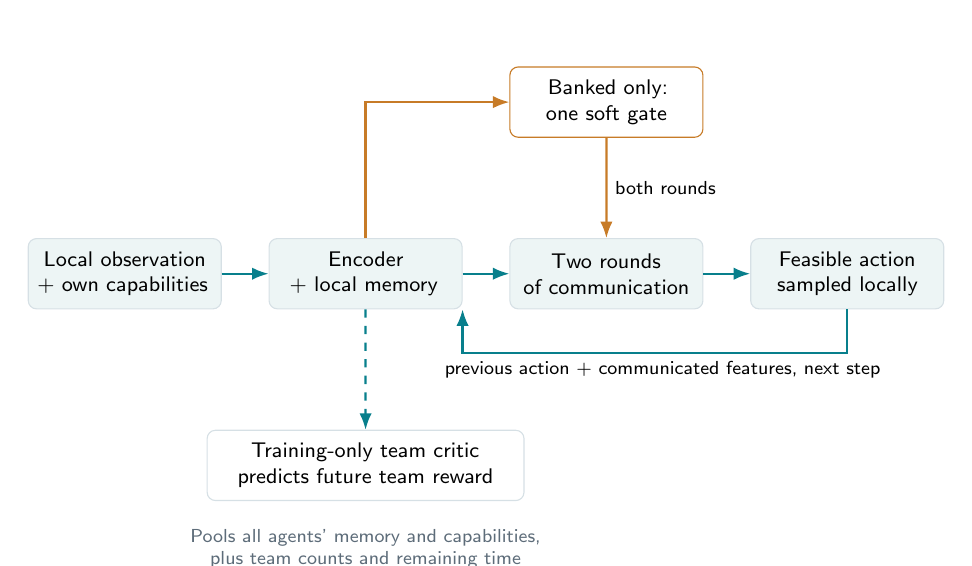
\begin{tikzpicture}[scale=.85,transform shape,box/.style={draw=line,fill=pale,rounded corners=3pt,align=center,text width=2.65cm,minimum height=1.05cm,font=\small},arr/.style={-{Latex[length=2.1mm]},thick,draw=teal}]
\node[box] (x) {Local observation\\+ own capabilities};
\node[box,right=7mm of x] (h) {Encoder\\+ local memory};
\node[box,right=7mm of h] (c) {Two rounds\\of communication};
\node[box,right=7mm of c] (a) {Feasible action\\sampled locally};
\draw[arr] (x)--(h);\draw[arr] (h)--(c);\draw[arr] (c)--(a);
\node[box,above=15mm of c,draw=amber,fill=white] (g) {Banked only:\\one soft gate};
\draw[arr,draw=amber] (h.north)|-(g.west);
\draw[arr,draw=amber] (g)--node[right,font=\footnotesize]{both rounds}(c);
\node[box,below=18mm of h,text width=4.5cm,fill=white] (v) {Training-only team critic\\predicts future team reward};
\draw[arr,dashed] (h)--(v);
\node[below=3mm of v,font=\footnotesize,align=center,text=muted] {Pools all agents' memory and capabilities,\\plus team counts and remaining time};
\draw[arr] (a.south)--++(0,-.65)-|node[pos=.24,below,font=\footnotesize,fill=white]{previous action + communicated features, next step}(h.south east);
\end{tikzpicture}
\end{center}

\sub{Read the diagram as a repeated cycle}
The agent summarizes its current view and combines it with memory. It sends a short message and weighs what it hears, twice, then chooses a possible action. Memory, communication features and action feed the next step. Past observations can influence decisions without assuming perfect recall.

The \textbf{critic} predicts how much team reward remains. It provides a training signal, like an estimate against which the outcome is compared. Its output never enters the actor's decision. Its loss can still improve the shared encoder and memory during training.

\sub{Three models, two different comparisons}
{\small\renewcommand{\arraystretch}{1.2}\begin{tabularx}{\linewidth}{@{}p{1.28in}XXX@{}}\toprule
 & HetNet Real & SoftRole shared & SoftRole banked \\\midrule
Information & Typed observations & Own abilities; merged agent counts & Same as shared \\
Communication & Class-dependent real vectors & One transform; binary messages & Four blended experts; binary messages \\
Learning path & Released learner & Team critic and team credit & Same as shared \\
Observation copies & Legacy behavior & Independent copies & Independent copies \\\bottomrule
\end{tabularx}}

\takeaway{Shared versus banked is our closest test of conditional communication weights. Banked also has more parameters. HetNet differs in several pipeline components.}
The network dimensions do not depend on team size. That makes new teams executable with the same weights; it does not guarantee successful transfer. No explicit P/A label or agent identity selects parameters in the new actor. Own capabilities still correlate with physical class in ordinary training.
\evidence{E2: \code{SoftRoleNet}, \code{CommunicationRound}, \code{adapt_observation}; original \code{hetgat/uavnet.py}. ``Independent copies'' prevent overlapping observation windows from accidentally modifying one another.}

\newpage
\pagetitle{03 / COMPONENTS}{What each part actually does}
\begingroup\normalsize
\textbf{1. Observation --- define what is knowable.} Each agent receives the existing position encoding, three sensory channels (outside-map, target, total number of agents), and two capability flags $\kappa=(\text{sense},\text{actuate})$. Agent \emph{counts} are added across classes, so two agents in one cell remain two. Neighbor class labels are removed. The input has 702 numbers in PP/PCP and 254 in FC. Losing sensing masks the three sensory channels; location information, movement, memory and radio remain. Own sensor health is supplied, not discovered by the policy.

\textbf{2. Encoder and LSTM --- summarize and remember.} A learned encoder reduces the input to 128 features. An LSTM, a neural network with memory, combines these with 16 previous communication features and six previous-action indicators. It maintains a 64-number hidden state and a 64-number internal memory state. The input width is $128+16+6=150$. This is a learned summary, not a guaranteed map of everything previously seen.

\textbf{3. Soft gate and banks --- blend communication weights.} In the banked model, memory and capabilities produce four nonnegative weights summing to one. For example, $(0.55,0.25,0.15,0.05)$ blends four expert transforms in those proportions:
\[
 B(x,g)=\sum_{k=1}^{4}g_k\bigl(W_kx+b_k\bigr),\qquad g_k\geq0,\quad \sum_k g_k=1.
\]
Here $x$ is a feature vector, $W_k$ and $b_k$ are an expert's learned matrix and bias, and $g_k$ is its mixing weight. One deterministic gate is computed per agent-step and reused in both rounds. ``Deterministic'' means the same inputs give the same gate; the messages and actions can still be random. The shared baseline uses one actual transform. Expert indices are not established semantic roles such as scout or rescuer.

\textbf{4. Binary messages and attention --- speak briefly, listen selectively.} Each round sends one 16-bit payload per agent. A learned score $u$ gives a bit a probability $\sigma(u)$ of being 1; $\sigma$ is the sigmoid function. The same sampled payload reaches all permitted receivers and all four attention heads. Heads are four learned ways of reading a message, not four extra transmissions. Encoding uses the sender's gate; decoding and attention use the receiver's gate. A zero-message ``null'' choice lets an agent allocate attention to no incoming information. With no neighbors the received aggregate is exactly zero. Round 1 produces 64 features; round 2 produces 16.

\textbf{5. Action head --- respect physical abilities.} The final 16 features produce probabilities for four moves, staying still, and capture/extinguish. If actuation is unavailable, the special action has exactly zero probability. The two rounds use \textbf{32 logical payload bits per agent-step}; that excludes packet headers and delivery overhead.

\textbf{6. Team critic and update --- learn from the whole team's outcome.} The critic averages agent features and adds team counts and remaining time, so permuting the roster does not change its prediction. Rewards are summed over physical agents. At each time step, all agents' action scores use the same team advantage: how much better or worse the outcome was than expected. Gradients, which indicate how to adjust learned weights, are summed across complete episodes, divided once by the global episode count, clipped once, then used for one RMSprop update.

\captiontext{Training settings: actor coefficient 50, value coefficient 1; discount $\gamma=1$; GAE $\lambda=0.95$; gradient paths cut every 5 steps, while memory is retained; learning rate $10^{-4}$; RMSprop $\alpha=0.97$, $\epsilon=10^{-6}$; clip norm 0.75. Binary backpropagation uses a biased straight-through sigmoid derivative. GAE with a learned critic and truncated recurrence are also approximations.}
\evidence{E2: \code{softrole/model.py}, \code{learning.py}, \code{train.py}, \code{config.py}. Current implementation uses deterministic gates; Gaussian roles, KL regularization and arrivals/departures within an episode are deferred.}
\endgroup

\newpage
\pagetitle{04 / READING THE EVIDENCE}{What the comparison can tell us}
The resynced snapshot contains \textbf{27 runs and 37,566 completed epochs}, adding 10,688 epochs to the earlier same-day logs. It covers three tasks, three models and three seeds per combination. A \textbf{seed} starts a separate randomized training run. The 18 SoftRole runs record 631,310,527 environment steps and zero exposed sensor failures. These are fixed-team runs; their curves do not test adaptation.

\textbf{Return} adds all agents' rewards across one episode; higher, including less negative, is better within a task. \textbf{Success} is the fraction of episodes meeting the task objective. \textbf{Episode length} counts steps until success or the time limit, including unsuccessful episodes. Read length with success: fewer steps alone is not sufficient evidence of improvement. An \textbf{epoch} groups ten optimizer updates here.

\sub{A contextual comparison at the same epoch window}
The following values average the last 50 epochs ending at the latest epoch available for \emph{every} run of a task. Epochs are weighted equally within each run; the three seeds then receive equal weight. These windows compare update counts, not equal samples or compute.
\par{\small\renewcommand{\arraystretch}{1.12}\begin{tabularx}{\linewidth}{@{}p{1.23in}Xrrr@{}}\toprule
Task / epochs & Model & Success (\%) & Return & Steps \\\midrule
PP / 343--392 & HetNet Real & 99.71 & -2.115 & 18.25 \\
PP / 343--392 & shared & 100.00 & -0.374 & 4.88 \\
PP / 343--392 & banked & 100.00 & -0.376 & 4.90 \\
\addlinespace[3pt]
PCP / 949--998 & HetNet Real & 99.59 & -2.112 & 17.94 \\
PCP / 949--998 & shared & 99.99 & -0.548 & 6.92 \\
PCP / 949--998 & banked & 99.99 & -0.638 & 8.61 \\
\addlinespace[3pt]
FC / 976--1025 & HetNet Real & 40.73 & -223.759 & 218.96 \\
FC / 976--1025 & shared & 64.37 & -143.426 & 184.44 \\
FC / 976--1025 & banked & 48.58 & -191.338 & 211.75 \\
\bottomrule
\end{tabularx}}
\captiontext{Rounding can show 100.00\% despite rare failures. Table values are changing-policy training statistics, not held-out evaluation scores. ``Steps'' here means episode length.}

\sub{Why the following plots use two horizontal axes}
HetNet's printed cumulative sample counters repeatedly add already-cumulative within-epoch totals. They therefore overcount. We use its valid completed-epoch axis. SoftRole's step and episode counts reconcile, so its plots use recorded environment steps. The two columns' horizontal positions are not equal training budgets.

For the closer \textbf{shared versus banked} comparison, pages 5--7 use the last 50 completed epochs at or before a common sample budget. Within each seed, an epoch with twice as many episodes receives twice the weight; the three seed estimates are then averaged equally. This pools episodes without letting a faster seed dominate. Endpoints fall less than 0.08\% below the stated budgets.

\takeaway{Observed progress is real in these logs. It does not isolate the effect of banks against HetNet, establish final convergence, or demonstrate robustness.}
The pipelines differ in observations, binary versus real communication, recurrence and learning. Three seed traces show variability; they are not confidence intervals. New stdout extends the older structured archive, but the corresponding newer checkpoints and source archives have not been supplied.
\evidence{E1: current raw logs re-parsed; old byte prefixes and archived metric/configuration identities verified. Per-run windows and grouped statistics independently recomputed. Source lines and exact windows are retained in the audit.}

\newpage
\pagetitle{05 / PREDATOR--PREY}{PP: strong learning, little separation}
\begingroup\fontsize{10.5}{12.5}\selectfont
Three sensing agents must all reach a stationary prey before 80 steps. This is the simplest nominal test: there is no separate actuation agent and no sensor loss.
\par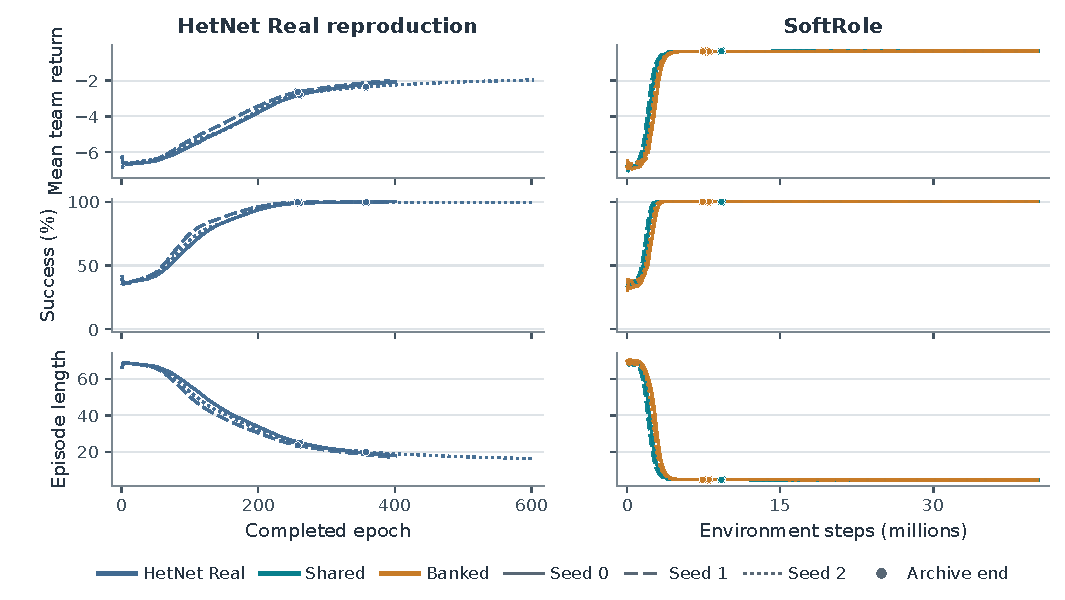
\includegraphics[width=\linewidth]{figures/pp_training.pdf}\par
\captiontext{Each line is one seed. Curves use trailing 50 epochs: equal-epoch means for HetNet; episode-weighted means for SoftRole. Dots mark the older structured-archive endpoint. Left and right use different training axes; see page 4.}
\sampletable{Shared & 99.999 & -0.356 & 4.74 \\
Banked & 99.995 & -0.357 & 4.75 \\
}{37}

\sub{What has improved}
Both SoftRole variants reach approximately 100\% training success and about 4.75 steps per episode. At the same 37M-step budget their returns and lengths are close: banked is about 0.01 steps longer on average. Additional training has changed this comparison very little.

The HetNet reproduction also reaches high success: its own latest 50-epoch windows average \textbf{99.75\%}, with return \textbf{$-2.009$} and length \textbf{17.21}, improving from 18.85 steps in the previous snapshot. These latest windows end at different epochs across seeds; page 4 gives the common-epoch comparison.

\takeaway{PP confirms that the implemented policies can learn the ordinary task. It supplies little evidence that four experts help beyond a shared transform.}
\evidence{E1: \code{summary.json}, task=\code{pp}, \code{common_sample} and \code{latest}; all three seeds. Raw stdout paths and line numbers are in \code{epoch_metrics.csv}.}
\endgroup

\newpage
\pagetitle{06 / PREDATOR--CAPTURE}{PCP: success catches up; speed differs}
\begingroup\fontsize{10.5}{12.5}\selectfont
Two sensing agents locate and reach the prey; one actuation agent must also reach and capture it. This is our primary domain for studying changed teams and sensor loss, although these training curves use the fixed, healthy team.
\par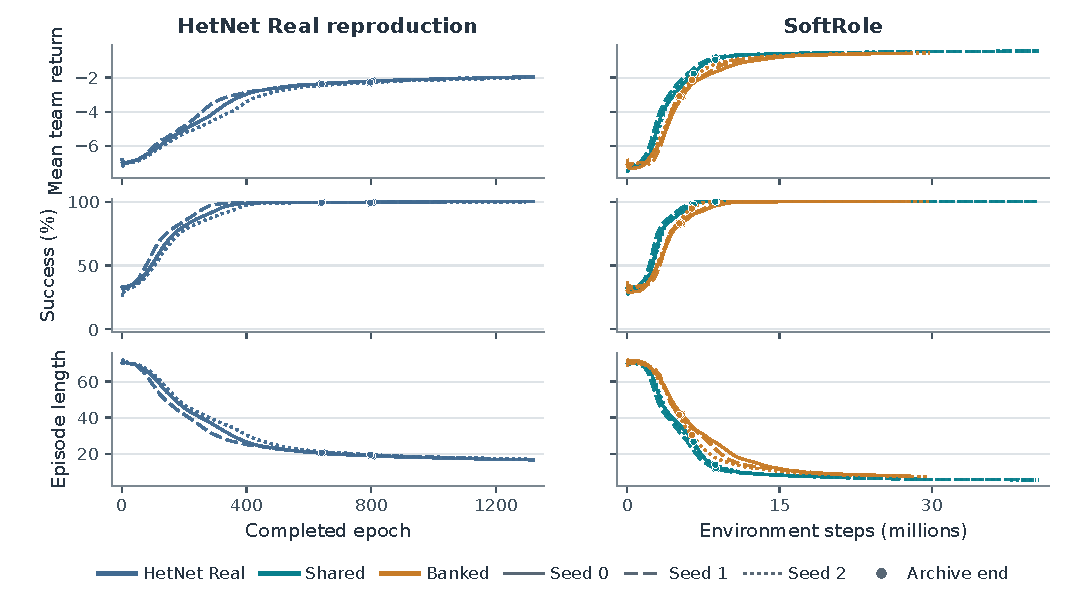
\includegraphics[width=\linewidth]{figures/pcp_training.pdf}\par
\captiontext{Each line is one seed; trailing 50-epoch means with the weighting from page 4. Dots mark the older archive endpoint. The runs end at different sample counts; the table compares a common budget.}
\sampletable{Shared & 99.995 & -0.552 & 7.00 \\
Banked & 99.989 & -0.645 & 8.75 \\
}{20}

\sub{The positive result and the remaining gap}
At the earlier 5M-step comparison, shared/banked success was \textbf{91.07\% / 81.89\%}. At 20M it is approximately 100\% for both, using the same episode-weighted method. Banked has largely closed the earlier success gap.

Shared remains faster: \textbf{7.00 versus 8.75 steps}, or \textbf{20.0\% fewer} using $1-7.0010/8.7523$. The gap has narrowed from 26.7\% at 15M. Seed lengths span 6.85--7.20 for shared and 8.43--8.96 for banked. Shared also earns the less-negative return. This is an observed efficiency advantage, not a significance claim.

HetNet's own latest windows average \textbf{99.88\%} success, return \textbf{$-2.003$}, and length \textbf{16.99}. Its task learning is clear; pipeline differences prevent assigning the gap to any single SoftRole component.
\takeaway{Banked learns nominal PCP successfully and the speed gap is narrowing. Shared retains the observed efficiency advantage at 20M steps.}
\evidence{E1: task=\code{pcp}, \code{prior_common_sample}, \code{common_sample}, per-run windows and \code{latest}. Reported speed reduction is a ratio of equal-seed mean episode lengths.}
\endgroup

\newpage
\pagetitle{07 / FIRECOMMANDER}{FC: progress with serious qualifications}
\begingroup\fontsize{10.5}{12.5}\selectfont
The team must extinguish all fire within 300 steps. The new logs show wide seed variation; a confirmed simulator defect also limits interpretation.
\par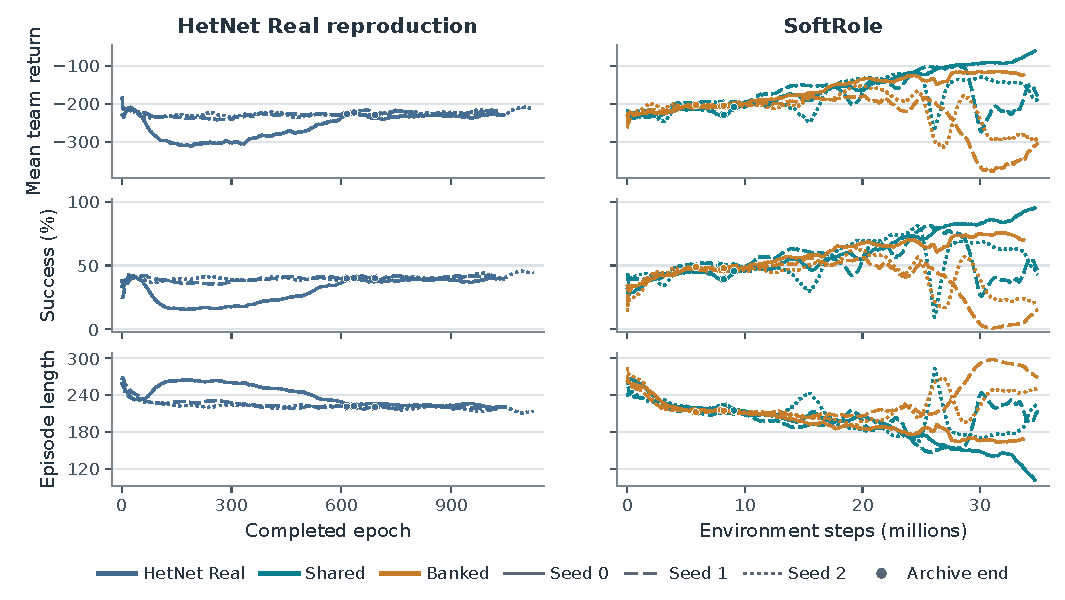
\includegraphics[width=\linewidth]{figures/fc_training.pdf}\par
\captiontext{Three seeds per variant; trailing 50-epoch means. Common-budget estimates below should not be replaced by the unequal-budget endpoints. Lower episode length includes failures at the 300-step limit.}
\sampletable{Shared & 63.91 & -143.273 & 178.35 \\
Banked & 32.97 & -251.131 & 233.31 \\
}{33.5}

At this budget, shared success is \textbf{30.94 percentage points higher}. Seed ranges are very broad: \textbf{39.45--90.67\%} for shared and \textbf{4.52--70.19\%} for banked. HetNet's latest windows average \textbf{41.98\%} success, return \textbf{$-219.862$}, and length \textbf{217.21}.

\textbf{The new tail exposes further instability.} Latest shared seed 0/1/2 success is \textbf{95.15/46.22/43.12\%}; banked is \textbf{69.92/15.53/19.90\%}. Banked seeds 1 and 2 regress substantially. Five FC SoftRole runs reach epoch 1,400; banked seed 0 ends at 1,354. These latest windows have unequal sample counts.

\textbf{Environment defect:} skipped boundary fronts create spurious origin fires and rewards. The prior audit found this placeholder in 945/1,000 passive resets by step 300 and 138/144 older frozen-policy outcomes. This limits physical interpretation; it does not establish the cause of the late regressions.
\takeaway{FC shows learning, variability and a simulator problem. It is not clean evidence of physical firefighting quality or a settled architecture ranking.}
\evidence{E1: FC common-budget and latest per-seed windows. E3: \code{simulator_probe.json} and \code{policy_panel/summary.json}. The earlier simulator/policy audit was not rerun for this document.}
\endgroup

\newpage
\pagetitle{08 / LEARNING DIAGNOSTICS}{What is happening inside training?}
\begingroup\fontsize{10.5}{12.5}\selectfont
Performance curves say whether behavior improves. The following diagnostics help locate changes in training, but they cannot by themselves identify why a policy succeeds or fails.
\par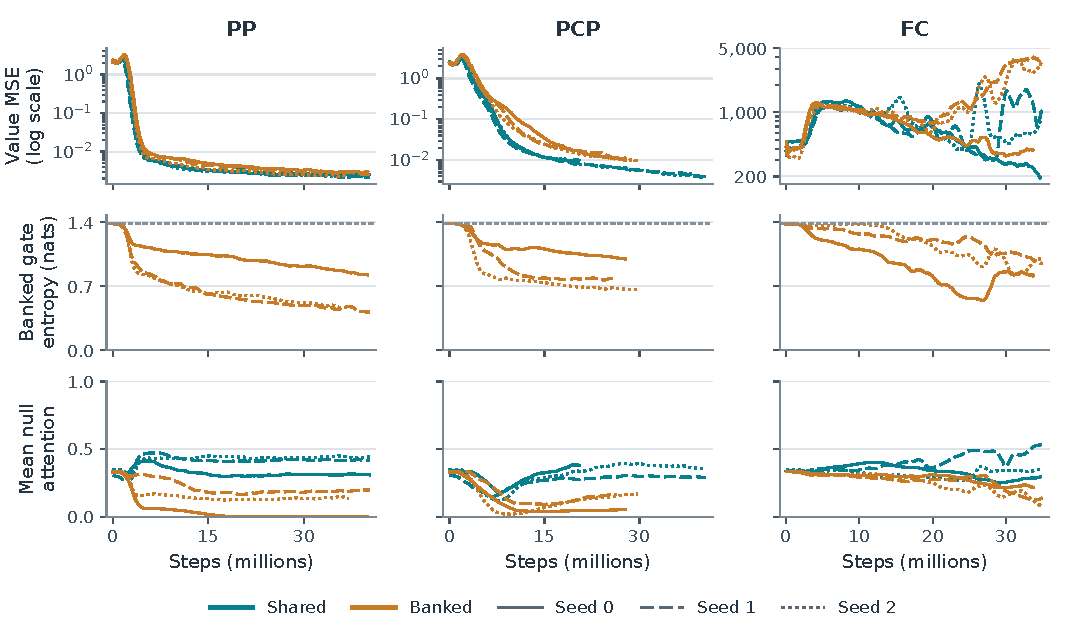
\includegraphics[width=\linewidth]{figures/diagnostics.pdf}\par
\captiontext{SoftRole only. Three seeds per variant; episode-weighted trailing 50-epoch means. Value error uses a logarithmic vertical scale. Gate entropy is shown only for banked; shared has one transform.}

\textbf{Value MSE: how far the critic is from its training target.} MSE means mean squared error: prediction errors are squared before averaging. Lower is closer to the current target, which itself depends on a learned critic and GAE. Latest FC banked seed 1/2 errors are about 3,609/3,642, alongside 15.53/19.90\% success. This association is a reason to inspect training, not proof that critic error caused the regressions.

\textbf{Gate entropy: how spread out the four expert weights are.} Zero would mean all weight on one expert; the maximum $\log 4\approx1.386$ means equal weights. A low value alone does not show useful specialization, and a high value does not show failure. The experts' learned transforms and actual policy behavior also matter.

\textbf{Null attention: how much attention goes to receiving zero.} Within each episode, it averages the no-message weight over steps, agents, rounds and heads; episodes then receive equal weight. An isolated receiver necessarily gives null all its weight. Nonzero attention to neighbors does not prove their messages cause better behavior; a matched communication-removal experiment is needed.

\takeaway{These diagnostics guide experiments; they do not prove roles, communication benefit or adaptation.}
\captiontext{Loss scales differ across pipelines and cannot rank policies. The latest SoftRole epoch logs omit action entropy and gradient norms; older audits do not supply current values.}
\evidence{E1: epoch fields \code{value_loss_per_episode}, \code{gate_entropy}, \code{alpha_null}, and latest FC per-seed windows. E2: their computation in \code{rollout.py} and \code{learning.py}.}
\endgroup

\newpage
\pagetitle{09 / ADAPTATION AND STATUS}{The main research question is still open}
The large training snapshot has \textbf{fixed teams and no sensor-loss exposure}. It establishes ordinary task learning. A separate, small PCP pilot checks the failure protocol and illustrates why success after a scheduled failure is not automatically evidence of recovery.

\sub{What the sensor-loss pilot actually did}
One nominally trained checkpoint per model, both seed 0, was chosen using the first archived checkpoint reaching 4M steps: shared had 4,265,196 steps, banked 4,279,220. Both were epoch 200. Twenty common scenarios scheduled one sensing-agent failure at a step from 10--30. Each had a matched \textbf{sham}: the same scenario, victim, event schedule and random streams, with sensor loss suppressed. Weights were frozen.

{\small\renewcommand{\arraystretch}{1.25}\begin{tabularx}{\linewidth}{@{}Xrrrr@{}}\toprule
 & Sham & Failure & Mean return & Exposed \\
Model & successes & successes & sham / failure & to loss \\\midrule
Shared & 15/20 & 14/20 & -3.2300 / -3.4575 & 15/20 \\
Banked & 15/20 & 16/20 & -3.6575 / -3.6350 & 18/20 \\
\bottomrule
\end{tabularx}}

Shared changes by --5 percentage points and banked by +5; each is \textbf{one scenario out of twenty}. That does not establish model superiority or a benefit from sensor loss. Some scenarios finish before the event: 5/20 shared and 2/20 banked. Thus the two policies experience loss on different subsets even though the assigned panel is the same.

Among exposed victims, \textbf{14/15 shared and 18/18 banked} had already directly seen the target; \textbf{8/15 and 11/18} had reached it. This pilot mostly removes sensing after discovery. Prior sight is not guaranteed retained knowledge, and an agent already at the target may still help through messages. Full-panel outcomes remain primary; exposed-only statistics need their denominators.

\sub{What is implemented, and what remains}
\textbf{Implemented:} shared and banked actors; three released tasks; variable rosters between episodes; PCP sensor loss; frozen evaluation with separate random streams; matched shams; event exposure and censoring; gate-freeze and communication-removal controls. Earlier engineering validation recorded 178 passing tests. Those tests check implementation behavior, not learned robustness.

\textbf{Next evidence needed:} run the locked multi-seed PCP failure-training comparison, test mechanism controls, then evaluate frozen weights on held-out teams without tuning to those outcomes. Prespecify any harder/earlier supplemental event using training compositions. Resync FC checkpoints near the regression and evaluate fixed scenarios. A physical FC correction should be explicitly versioned and studied separately.

\textbf{Deferred:} Gaussian latent roles and KL penalties, arrivals/departures during an episode, physical FC sensor-loss semantics, and formal paired seed-level inference. The code's ability to execute a changed team is not a result about performance on that team.
\takeaway{Current evidence supports a working, auditable system and strong nominal PP/PCP learning. The added value of banks for capability changes remains an experimental question.}
\evidence{E4: the 20-scenario pilot's manifests, paired reports and summary. E5: prior 178-test validation; no training, evaluation or runtime test suite was launched to prepare this PDF.}

\newpage
\pagetitle{10 / TRACEABILITY}{How to check every result}
This document uses the latest local logs available on 30 September 2026. All inputs were read without modification. The accompanying folder contains editable LaTeX, figure code, exact comparison values, raw-log checks, evidence mappings and SHA256 hashes (fingerprints that detect changed files).

\sub{Snapshot coverage}
{\small\renewcommand{\arraystretch}{1.05}\begin{tabularx}{\linewidth}{@{}lXrr@{}}\toprule
Task & Model (three seeds each) & Last epoch range & SoftRole steps (M) \\\midrule
PP & HetNet Real & 392--603 & -- \\
PP & SoftRole shared & 2000--2000 & 40.29--40.30 \\
PP & SoftRole banked & 1837--2000 & 37.04--40.32 \\
PCP & HetNet Real & 1113--1320 & -- \\
PCP & SoftRole shared & 998--1998 & 20.45--40.52 \\
PCP & SoftRole banked & 1287--1455 & 26.40--29.73 \\
FC & HetNet Real & 1025--1125 & -- \\
FC & SoftRole shared & 1400--1400 & 34.64--34.89 \\
FC & SoftRole banked & 1354--1400 & 33.70--34.98 \\
\bottomrule
\end{tabularx}}
\captiontext{Ranges describe three endpoints, not uncertainty intervals. HetNet's new cumulative stdout sample counts are not usable. Nine runs reach their configured targets: four SoftRole PP and five SoftRole FC. Targets are 2,000 epochs for PP/PCP and 1,400 for FC; reaching them is not proof of convergence.}

\sub{Local evidence map}
{\fontsize{9}{11}\selectfont
\textbf{E1 --- current training.} \code{logs_1/*.out}, \code{logs_sr/*.out}; this document's \code{latest_snapshot/{summary.json,epoch_metrics.csv,provenance.json}}. Each summary run names its raw log; the CSV names its source line. \code{review_results.json} checks raw values and arithmetic. Earlier comparisons use \code{analysis/training_2026-09-30_resync/summary.json}.

\textbf{E2 --- architecture and metrics.} \code{softrole/{env,model,learning,rollout,train,config}.py}, \code{softrole/RESEARCH.md}, original model and simulator sources. \code{evidence_index.json} expands paths and lookup instructions.

\textbf{E3 --- FC audit.} \code{analysis/fc_audit_2026-09-30/}: \code{simulator_probe.json}, \code{log_findings.json}, \code{policy_panel/summary.json}. These preserve the earlier diagnostic panels; they are separate from the newer training tail.

\textbf{E4 --- sensor pilot.} \code{runs/sensor_failure_validation_20260930/pilot/}: \code{pilot.json}, \code{scenarios.json}, \code{summary.json} and four condition reports. \textbf{E5 --- engineering record.} Repository \code{AGENTS.md}; dated checks are not represented as newly executed experiments.
}

\sub{Primary references}
{\fontsize{9}{11}\selectfont
[1] Seraj et al. (2022), \href{https://ifaamas.org/Proceedings/aamas2022/pdfs/p1173.pdf}{\emph{Learning Efficient Diverse Communication for Cooperative Heterogeneous Teaming}}. AAMAS.\par
[2] Howell et al. (2023), \href{https://proceedings.mlr.press/v229/howell23a.html}{\emph{Generalization of Heterogeneous Multi-Robot Policies via Awareness and Communication of Capabilities}}. CoRL.\par
[3] Fu et al. (2025), \href{https://arxiv.org/abs/2501.06058}{\emph{Capability-Aware Shared Hypernetworks for Flexible Heterogeneous Multi-Robot Coordination}}. CASH.\par
[4] Brody et al. (2022), \href{https://arxiv.org/abs/2105.14491}{\emph{How Attentive are Graph Attention Networks?}} GATv2.\par
[5] Schulman et al. (2016), \href{https://arxiv.org/abs/1506.02438}{\emph{High-Dimensional Continuous Control Using Generalized Advantage Estimation}}.\par
[6] Zaheer et al. (2017), \href{https://papers.nips.cc/paper/2017/hash/f22e4747da1aa27e363d86d40ff442fe-Abstract.html}{\emph{Deep Sets}}. Permutation-invariant aggregation.\par
[7] Agarwal et al. (2021), \href{https://arxiv.org/abs/2108.13264}{\emph{Deep Reinforcement Learning at the Edge of the Statistical Precipice}}. Evaluation uncertainty; motivates caution with a few runs.
}
\evidence{All paper links are clickable. \code{input_manifest.json} records local input identities; \code{comparison_values.csv} gives unrounded numbers; \code{validation.json} records this document's build and checks. No new performance experiments are presented.}
\end{document}
